% Options for packages loaded elsewhere
\PassOptionsToPackage{unicode}{hyperref}
\PassOptionsToPackage{hyphens}{url}
\PassOptionsToPackage{dvipsnames,svgnames,x11names}{xcolor}
%
\documentclass[
  12pt,
  a4paper, twoside]{book}
\usepackage{amsmath,amssymb}
\usepackage{lmodern}
\usepackage{iftex}
\ifPDFTeX
  \usepackage[T1]{fontenc}
  \usepackage[utf8]{inputenc}
  \usepackage{textcomp} % provide euro and other symbols
\else % if luatex or xetex
  \usepackage{unicode-math}
  \defaultfontfeatures{Scale=MatchLowercase}
  \defaultfontfeatures[\rmfamily]{Ligatures=TeX,Scale=1}
\fi
% Use upquote if available, for straight quotes in verbatim environments
\IfFileExists{upquote.sty}{\usepackage{upquote}}{}
\IfFileExists{microtype.sty}{% use microtype if available
  \usepackage[]{microtype}
  \UseMicrotypeSet[protrusion]{basicmath} % disable protrusion for tt fonts
}{}
\makeatletter
\@ifundefined{KOMAClassName}{% if non-KOMA class
  \IfFileExists{parskip.sty}{%
    \usepackage{parskip}
  }{% else
    \setlength{\parindent}{0pt}
    \setlength{\parskip}{6pt plus 2pt minus 1pt}}
}{% if KOMA class
  \KOMAoptions{parskip=half}}
\makeatother
\usepackage{xcolor}
\IfFileExists{xurl.sty}{\usepackage{xurl}}{} % add URL line breaks if available
\IfFileExists{bookmark.sty}{\usepackage{bookmark}}{\usepackage{hyperref}}
\hypersetup{
  pdflang={fi},
  colorlinks=true,
  linkcolor={blue},
  filecolor={Maroon},
  citecolor={blue},
  urlcolor={blue},
  pdfcreator={LaTeX via pandoc}}
\urlstyle{same} % disable monospaced font for URLs
\usepackage{longtable,booktabs,array}
\usepackage{calc} % for calculating minipage widths
% Correct order of tables after \paragraph or \subparagraph
\usepackage{etoolbox}
\makeatletter
\patchcmd\longtable{\par}{\if@noskipsec\mbox{}\fi\par}{}{}
\makeatother
% Allow footnotes in longtable head/foot
\IfFileExists{footnotehyper.sty}{\usepackage{footnotehyper}}{\usepackage{footnote}}
\makesavenoteenv{longtable}
\usepackage{graphicx}
\makeatletter
\def\maxwidth{\ifdim\Gin@nat@width>\linewidth\linewidth\else\Gin@nat@width\fi}
\def\maxheight{\ifdim\Gin@nat@height>\textheight\textheight\else\Gin@nat@height\fi}
\makeatother
% Scale images if necessary, so that they will not overflow the page
% margins by default, and it is still possible to overwrite the defaults
% using explicit options in \includegraphics[width, height, ...]{}
\setkeys{Gin}{width=\maxwidth,height=\maxheight,keepaspectratio}
% Set default figure placement to htbp
\makeatletter
\def\fps@figure{htbp}
\makeatother
\setlength{\emergencystretch}{3em} % prevent overfull lines
\providecommand{\tightlist}{%
  \setlength{\itemsep}{0pt}\setlength{\parskip}{0pt}}
\setcounter{secnumdepth}{5}
\ifLuaTeX
\usepackage[bidi=basic]{babel}
\else
\usepackage[bidi=default]{babel}
\fi
\babelprovide[main,import]{finnish}
% get rid of language-specific shorthands (see #6817):
\let\LanguageShortHands\languageshorthands
\def\languageshorthands#1{}
\usepackage{booktabs}
\usepackage[T1]{fontenc}
\usepackage[utf8]{inputenc}
\usepackage{color}
\usepackage{xspace}
\usepackage{tikz-cd}
\usepackage{mathtools}
\usepackage{mathrsfs}
\usepackage{commath}
\usepackage{pict2e}
\usepackage{float}
\usepackage{array, makecell}
\usepackage{amsthm}														% 
\usepackage{amsmath}
%\usepackage[tagpdf]{axessibility} 
\usepackage[ruled,vlined,shortend]{algorithm2e} 
\usepackage{graphicx}
\usepackage{multicol}
\usepackage{gensymb}
%\usepackage[a-3b]{pdfx}
\graphicspath{ {./images/} }
\usetikzlibrary{shapes.geometric,arrows}
\def\TikZ{Ti\emph{k}Z\ }
\renewcommand{\algorithmcfname}{Algoritmi}
\usepackage{geometry}
\geometry{
    a4paper,
    total={150mm,237mm},
    left=30mm,
    top=30mm,
    }
\newcommand{\tekija}{{Lasse Rintakumpu}}
\newcommand{\titteli}{{}} 
\newcommand{\otsikko}{{SMC-menetelmät sekä niiden soveltaminen AoA-menetelmään perustuvassa sisätilapaikannuksessa}} 
\newcommand{\tutkielma}{{Pro gradu }}
\newcommand{\aika}{{Tammikuu 2023}} 
\newcommand{\paaaine}{{Tilastotiede}} 
\newcommand{\ohjaaja}{{Ohjaajan titteli (Prof./Dos./FT) ja nimi }} %
\newcommand{\tarkastaja}{{Toisen tarkastajan titteli (Prof./Dos./FT) ja nimi}} 
\ifLuaTeX
  \usepackage{selnolig}  % disable illegal ligatures
\fi
\usepackage[]{natbib}
\bibliographystyle{plainnat}

\author{}
\date{\vspace{-2.5em}}

\usepackage{amsthm}
\newtheorem{theorem}{Theorem}[chapter]
\newtheorem{lemma}{Lemma}[chapter]
\newtheorem{corollary}{Corollary}[chapter]
\newtheorem{proposition}{Proposition}[chapter]
\newtheorem{conjecture}{Conjecture}[chapter]
\theoremstyle{definition}
\newtheorem{definition}{Definition}[chapter]
\theoremstyle{definition}
\newtheorem{example}{Example}[chapter]
\theoremstyle{definition}
\newtheorem{exercise}{Exercise}[chapter]
\theoremstyle{definition}
\newtheorem{hypothesis}{Hypothesis}[chapter]
\theoremstyle{remark}
\newtheorem*{remark}{Remark}
\newtheorem*{solution}{Solution}
\begin{document}

\pagenumbering{roman}
\pagestyle{empty}

\begin{center}

\includegraphics[width=10cm]{UTU_logo_FI}
\end{center}

\vspace{3.0cm}
\begin{center}\large
{\sc \otsikko} 
\end{center}

\vspace{0.5cm}
\begin{center}
\titteli \tekija
\end{center}

\vspace{0.5cm}
\begin{center}
\tutkielma -tutkielma\\
\aika
\end{center}

\vspace{2.5cm}
\begin{center}
\begin{tabular}{l}
Tarkastajat:\\
\ohjaaja \\
\tarkastaja
\end{tabular}
\end{center}

\vspace{2.5cm}
\begin{center}
MATEMATIIKAN JA TILASTOTIETEEN LAITOS
\end{center}

\newpage\null

\vspace{22cm}

\noindent Turun yliopiston laatujärjestelmän mukaisesti tämän julkaisun alkuperäisyys on tarkastettu Turnitin OriginalityCheck-järjestelmällä

\cleardoublepage

\noindent
TURUN YLIOPISTO \newline
Matematiikan ja tilastotieteen laitos\newline

\noindent \textsc{\tekija}: \otsikko \newline
\tutkielma-tutkielma, X s. \newline
\paaaine \newline
\aika
\par\noindent{\rule{\textwidth}{.2mm}} \newline


\vspace{4mm}\noindent Tutkielmassa esitetään sekventiaalisten Monte Carlo -menetelmien (SMC) teoria Bayesilaisessa tilastotieteellisessä viitekehyksessä. LISÄKSI

\vspace{4mm}\noindent Empiirisenä esimerkkinä tutkielmassa tarkastellaan SMC-menetelmien käyttöä AoA-teknologiaan perustuvassa sisätilapaikannusratkaisussa.

\vspace{4mm}\noindent Asiasanat: SMC-menetelmät, Monte Carlo -menetelmät, sekventiaalinen Monte Carlo, suodinongelma, hiukassuodin, SIR-algoritmi, sisätilapaikannus, BLE, AoA, triangulaatio, Bayesilainen päättely

\cleardoublepage

\cleardoublepage

\pagestyle{plain} 
\pagenumbering{arabic} 

{
\hypersetup{linkcolor=blue}
\setcounter{tocdepth}{2}
\tableofcontents
}
\setlength\parindent{24pt}
\setlength\parskip{3pt}

\hypertarget{johdanto}{%
\chapter{Johdanto}\label{johdanto}}

Lorem ipsum.

\hypertarget{notaatioista}{%
\section{Notaatioista}\label{notaatioista}}

Lorem ipsum.

\hypertarget{suodin--ja-siloitteluongelmat}{%
\section{Suodin- ja siloitteluongelmat}\label{suodin--ja-siloitteluongelmat}}

Lorem ipsum.

\hypertarget{suodin--ja-siloitteluongelmien-historiaa}{%
\section{Suodin- ja siloitteluongelmien historiaa}\label{suodin--ja-siloitteluongelmien-historiaa}}

Lorem ipsum.

\hypertarget{monte-carlo--menetelmistuxe4}{%
\chapter{Monte Carlo -menetelmistä}\label{monte-carlo--menetelmistuxe4}}

\hypertarget{monte-carlo--menetelmien-historiaa}{%
\section{Monte Carlo -menetelmien historiaa}\label{monte-carlo--menetelmien-historiaa}}

\hypertarget{monte-carlo--approksimaatio}{%
\section{Monte Carlo -approksimaatio}\label{monte-carlo--approksimaatio}}

\hypertarget{tuxe4rkeytysotanta}{%
\section{Tärkeytysotanta}\label{tuxe4rkeytysotanta}}

\hypertarget{sekventiaalinen-monte-carlo}{%
\section{Sekventiaalinen Monte Carlo}\label{sekventiaalinen-monte-carlo}}

\hypertarget{bayesilainen-suodin-ja-siloitin}{%
\chapter{Bayesilainen suodin ja siloitin}\label{bayesilainen-suodin-ja-siloitin}}

Cross-references make it easier for your readers to find and link to elements in your book.

\hypertarget{bayesilainen-suodin}{%
\section{Bayesilainen suodin}\label{bayesilainen-suodin}}

There are two steps to cross-reference any heading:

\begin{enumerate}
\def\labelenumi{\arabic{enumi}.}
\tightlist
\item
  Label the heading: \texttt{\#\ Hello\ world\ \{\#nice-label\}}.

  \begin{itemize}
  \tightlist
  \item
    Leave the label off if you like the automated heading generated based on your heading title: for example, \texttt{\#\ Hello\ world} = \texttt{\#\ Hello\ world\ \{\#hello-world\}}.
  \item
    To label an un-numbered heading, use: \texttt{\#\ Hello\ world\ \{-\#nice-label\}} or \texttt{\{\#\ Hello\ world\ .unnumbered\}}.
  \end{itemize}
\item
  Next, reference the labeled heading anywhere in the text using \texttt{\textbackslash{}@ref(johdanto)};

  \begin{itemize}
  \tightlist
  \item
    If you prefer text as the link instead of a numbered reference use: \protect\hyperlink{johdanto}{any text you want can go here}.
  \end{itemize}
\end{enumerate}

\hypertarget{bayesilainen-siloitin}{%
\section{Bayesilainen siloitin}\label{bayesilainen-siloitin}}

Figures and tables \emph{with captions} can also be cross-referenced from elsewhere in your book using \texttt{\textbackslash{}@ref(fig:chunk-label)} and \texttt{\textbackslash{}@ref(tab:chunk-label)}, respectively.

See Figure \ref{fig:nice-fig}.

\begin{figure}

{\centering 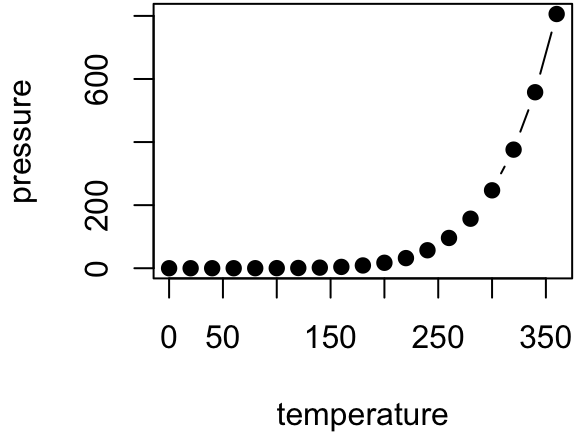
\includegraphics[width=0.8\linewidth]{output/figures/nice-fig-1} 

}

\caption{Here is a nice figure!}\label{fig:nice-fig}
\end{figure}

Don't miss Table \ref{tab:nice-tab}.

\begin{longtable}[]{@{}rr@{}}
\caption{Here is a nice table!}\tabularnewline
\toprule
temperature & pressure \\
\midrule
\endfirsthead
\toprule
temperature & pressure \\
\midrule
\endhead
0 & 0.0002 \\
20 & 0.0012 \\
40 & 0.0060 \\
60 & 0.0300 \\
80 & 0.0900 \\
100 & 0.2700 \\
120 & 0.7500 \\
140 & 1.8500 \\
160 & 4.2000 \\
180 & 8.8000 \\
\bottomrule
\end{longtable}

\hypertarget{kalman-suotimen-ja-hiukassuotimen-eroista}{%
\section{Kalman-suotimen ja hiukassuotimen eroista}\label{kalman-suotimen-ja-hiukassuotimen-eroista}}

\hypertarget{hiukkassuotimet}{%
\chapter{Hiukkassuotimet}\label{hiukkassuotimet}}

Add an appendix as a special kind of un-numbered part: \texttt{\#\ (APPENDIX)\ Other\ stuff\ \{-\}} (followed by \texttt{\#\ A\ chapter}). Chapters in an appendix are prepended with letters instead of numbers.

\hypertarget{saapasremmisuodin}{%
\section{Saapasremmisuodin}\label{saapasremmisuodin}}

Lorem ipsum

\hypertarget{sir-algoritmi}{%
\section{SIR-algoritmi}\label{sir-algoritmi}}

Lorem ipsum

\hypertarget{interpolaatiosta}{%
\subsection{Interpolaatiosta}\label{interpolaatiosta}}

Lorem ipsum

\hypertarget{parametrien-valinta}{%
\subsection{Parametrien valinta}\label{parametrien-valinta}}

Lorem ipsum

\hypertarget{marginaalijakauma}{%
\subsection{Marginaalijakauma}\label{marginaalijakauma}}

Lorem ipsum

\hypertarget{aikakompleksisuus}{%
\subsection{Aikakompleksisuus}\label{aikakompleksisuus}}

Lorem ipsum

\hypertarget{konvergenssituloksia}{%
\subsection{Konvergenssituloksia}\label{konvergenssituloksia}}

Lorem ipsum

\hypertarget{hiukkasiloittimet}{%
\chapter{Hiukkasiloittimet}\label{hiukkasiloittimet}}

Add an appendix as a special kind of un-numbered part: \texttt{\#\ (APPENDIX)\ Other\ stuff\ \{-\}} (followed by \texttt{\#\ A\ chapter}). Chapters in an appendix are prepended with letters instead of numbers.

\hypertarget{offline-algoritmit}{%
\section{Offline-algoritmit}\label{offline-algoritmit}}

Lorem ipsum

\hypertarget{sir-siloitin}{%
\subsection{SIR-siloitin}\label{sir-siloitin}}

\hypertarget{online-algoritmit}{%
\section{Online-algoritmit}\label{online-algoritmit}}

Lorem ipsum

\hypertarget{aoa-menetelmistuxe4}{%
\chapter{AoA-menetelmistä}\label{aoa-menetelmistuxe4}}

\hypertarget{music-algoritmi}{%
\section{MUSIC-algoritmi}\label{music-algoritmi}}

Footnotes are put inside the square brackets after a caret \texttt{\^{}{[}{]}}. Like this one \footnote{This is a footnote.}.

Citations. Reference items in your bibliography file(s) using \texttt{@key}.

For example, we are using the \textbf{bookdown} package \citep{R-bookdown} (check out the last code chunk in index.Rmd to see how this citation key was added) in this sample book, which was built on top of R Markdown and \textbf{knitr} \citep{xie2015} (this citation was added manually in an external file book.bib).
Note that the \texttt{.bib} files need to be listed in the index.Rmd with the YAML \texttt{bibliography} key.

The RStudio Visual Markdown Editor can also make it easier to insert citations: \url{https://rstudio.github.io/visual-markdown-editing/\#/citations}

\hypertarget{smc-menetelmuxe4t-sisuxe4tilapaikannuksessa}{%
\chapter{SMC-menetelmät sisätilapaikannuksessa}\label{smc-menetelmuxe4t-sisuxe4tilapaikannuksessa}}

\hypertarget{teknologian-kuvaus}{%
\section{Teknologian kuvaus}\label{teknologian-kuvaus}}

Here is an equation.

\begin{equation} 
  f\left(k\right) = \binom{n}{k} p^k\left(1-p\right)^{n-k}
  \label{eq:binom}
\end{equation}

You may refer to using \texttt{\textbackslash{}@ref(eq:binom)}, like see Equation \eqref{eq:binom}.

\hypertarget{koeasetelma}{%
\section{Koeasetelma}\label{koeasetelma}}

Labeled theorems can be referenced in text using \texttt{\textbackslash{}@ref(thm:tri)}, for example, check out this smart theorem \ref{thm:tri}.

\begin{theorem}
\protect\hypertarget{thm:tri}{}\label{thm:tri}For a right triangle, if \(c\) denotes the \emph{length} of the hypotenuse
and \(a\) and \(b\) denote the lengths of the \textbf{other} two sides, we have
\[a^2 + b^2 = c^2\]
\end{theorem}

Read more here \url{https://bookdown.org/yihui/bookdown/markdown-extensions-by-bookdown.html}.

\hypertarget{datan-kuvaus}{%
\section{Datan kuvaus}\label{datan-kuvaus}}

\hypertarget{ongelman-kuvaus}{%
\section{Ongelman kuvaus}\label{ongelman-kuvaus}}

\hypertarget{uskottavuusmalli}{%
\subsection{Uskottavuusmalli}\label{uskottavuusmalli}}

\hypertarget{dynaaminen-malli}{%
\subsection{Dynaaminen malli}\label{dynaaminen-malli}}

\hypertarget{algoritmien-toteutuksesta}{%
\section{Algoritmien toteutuksesta}\label{algoritmien-toteutuksesta}}

\hypertarget{parametrien-valinnasta}{%
\section{Parametrien valinnasta}\label{parametrien-valinnasta}}

\hypertarget{tulokset}{%
\section{Tulokset}\label{tulokset}}

\hypertarget{lopuksi}{%
\chapter{Lopuksi}\label{lopuksi}}

Lorem ipsum

\hypertarget{appendix-other-stuff--followed-by-a-chapter}{%
\chapter{\texorpdfstring{(APPENDIX) Other stuff \{-\}\texttt{(followed\ by}\# A chapter`)}{(APPENDIX) Other stuff \{-\}(followed by\# A chapter`)}}\label{appendix-other-stuff--followed-by-a-chapter}}

\hypertarget{appendix-other-stuff--followed-by-a-chapter-1}{%
\section{\texorpdfstring{(APPENDIX) Other stuff \{-\}\texttt{(followed\ by}\# A chapter`)}{(APPENDIX) Other stuff \{-\}(followed by\# A chapter`)}}\label{appendix-other-stuff--followed-by-a-chapter-1}}

  \bibliography{book.bib,packages.bib}

\end{document}
